\chapter{Amplitude-Shift Keying (ASK)}
\label{ch:ask}

\begin{nontechnical}
\textbf{ASK is like using a dimmer switch on a flashlight}---bright = 1, dim = 0. Simple to understand, but noise makes it hard to tell bright from dim!


\textbf{Simple idea:}
\begin{itemize}
\item Bit 0 = low amplitude (dim or off)
\item Bit 1 = high amplitude (bright)
\end{itemize}

\textbf{Real use:} Fiber optics uses On-Off Keying (binary ASK) at 10--100~Gbps. RFID tags use ASK for simple, low-power communication.

\textbf{Why amplitude-based is problematic:} Noise and fading directly affect amplitude, making it hard to distinguish signal levels. Phase (PSK) and frequency (FSK) modulation are more robust. Trade-off: Simple implementation but poor noise immunity compared to phase-based schemes.
\end{nontechnical}

\section{Overview}

\textbf{Amplitude-Shift Keying (ASK)} encodes digital data by varying the \textbf{amplitude} of a carrier wave while maintaining constant phase and frequency.

\begin{keyconcept}
ASK is the simplest form of digital modulation but suffers from \textbf{poor noise immunity} because noise directly affects amplitude. It is primarily used in \textbf{optical communications} (fiber optics) where the channel has inherently low noise, and in \textbf{RFID systems} where simplicity is paramount.
\end{keyconcept}

ASK modulation maps digital symbols to different amplitude levels. For M-ary ASK with $M$ distinct amplitude levels, each symbol carries $\log_2(M)$ bits of information. On-Off Keying (OOK) is the special case of binary ASK ($M=2$) where one amplitude is typically zero.

\section{Mathematical Description}

\subsection{Time-Domain Signal}

The general M-ary ASK waveform is expressed as:
\begin{equation}
s_m(t) = A_m \cos(2\pi f_c t), \quad 0 \leq t < T_s, \quad m = 0, 1, \ldots, M-1
\end{equation}
where:
\begin{itemize}
\item $A_m$ = amplitude level for symbol $m$
\item $f_c$ = carrier frequency (Hz)
\item $T_s$ = symbol period (seconds)
\item $M$ = number of distinct amplitude levels
\end{itemize}

\subsection{Binary ASK (2-ASK)}

For binary ASK with two amplitude levels $A_1$ and $A_2$ (typically 0 and $A$):
\begin{equation}
s(t) = \begin{cases}
A \cos(2\pi f_c t) & \text{if bit = 1} \\
0 & \text{if bit = 0}
\end{cases}
\end{equation}

This special case is called \textbf{On-Off Keying (OOK)} and is the most widely used form of ASK in practical systems.

\subsection{M-ary ASK}

For higher-order ASK, amplitude levels are typically equally spaced:
\begin{equation}
A_m = A_0 + m \cdot \Delta A
\end{equation}
where:
\begin{itemize}
\item $A_0$ = minimum amplitude (often 0)
\item $\Delta A$ = amplitude spacing between levels
\item $m$ = symbol index ($0$ to $M-1$)
\end{itemize}

\textbf{Bits per symbol:}
\begin{equation}
\text{Bits/symbol} = \log_2(M)
\end{equation}

\section{IQ Representation}

The baseband complex representation of ASK is:
\begin{equation}
s(t) = \mathrm{Re}\{A_m \cdot e^{j2\pi f_c t}\}
\end{equation}

\textbf{IQ components:}
\begin{itemize}
\item \textbf{I (In-phase):} $I_m = A_m$ (varies with symbol)
\item \textbf{Q (Quadrature):} $Q_m = 0$ (ASK uses only the I axis)
\end{itemize}

\subsection{Constellation Diagram}

ASK constellation points lie on a single dimension (the real/I axis) since only amplitude varies:

\begin{center}
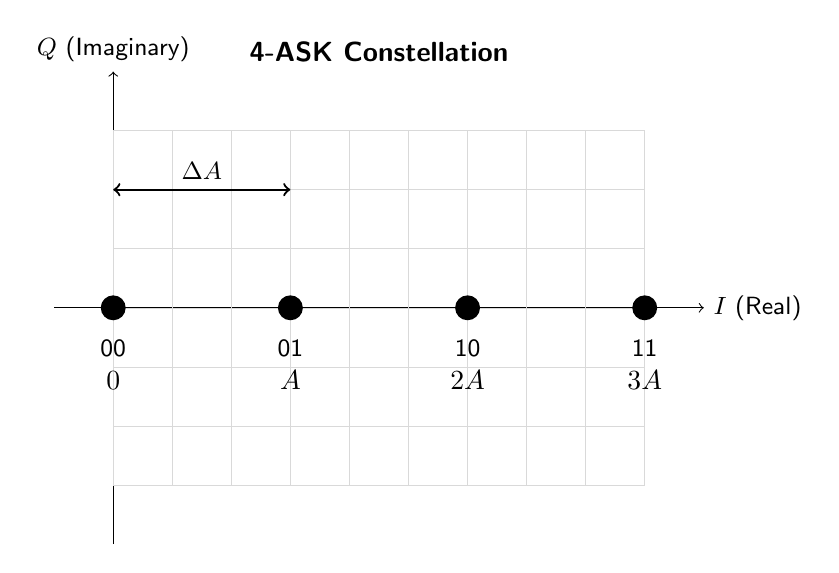
\begin{tikzpicture}[scale=1.5]
% Axes
\draw[->] (-0.5,0) -- (5,0) node[right] {\sffamily\small $I$ (Real)};
\draw[->] (0,-2) -- (0,2) node[above] {\sffamily\small $Q$ (Imaginary)};

% Grid
\draw[very thin,gray!30] (0,-1.5) grid[step=0.5] (4.5,1.5);

% 4-ASK Constellation points
\fill[black] (0,0) circle (3pt);
\fill[black] (1.5,0) circle (3pt);
\fill[black] (3,0) circle (3pt);
\fill[black] (4.5,0) circle (3pt);

% Labels
\node[below=8pt,align=center] at (0,0) {\sffamily\small 00\\$0$};
\node[below=8pt,align=center] at (1.5,0) {\sffamily\small 01\\$A$};
\node[below=8pt,align=center] at (3,0) {\sffamily\small 10\\$2A$};
\node[below=8pt,align=center] at (4.5,0) {\sffamily\small 11\\$3A$};

% Distance annotation
\draw[<->,thick] (0,1) -- (1.5,1) node[midway,above] {\sffamily\small $\Delta A$};

\node[above,font=\sffamily\bfseries] at (2.25,2) {4-ASK Constellation};
\end{tikzpicture}
\end{center}

\textbf{Key observations:}
\begin{itemize}
\item All constellation points lie on the I-axis ($Q = 0$)
\item Minimum distance between adjacent points: $d_{\min} = \Delta A$
\item Unlike 2D modulation (QAM, PSK), 1D arrangement is inherently less power-efficient
\item Noise must exceed $\Delta A/2$ to cause a symbol error
\end{itemize}

\begin{calloutbox}[colback=black!5!white,colframe=black]{4-ASK Example}
\textbf{Parameters:}
\begin{itemize}
\item Four amplitude levels: $0, A, 2A, 3A$
\item Bits per symbol: $\log_2(4) = 2$ bits
\item Symbol mapping: 00$\rightarrow$0, 01$\rightarrow A$, 10$\rightarrow 2A$, 11$\rightarrow 3A$
\item Spectral efficiency: 2 bits/symbol (double that of binary ASK)
\end{itemize}
\end{calloutbox}

\section{Modulation and Demodulation}

\subsection{Transmitter (Modulator)}

The ASK modulator generates amplitude-modulated carrier signals:

\begin{center}
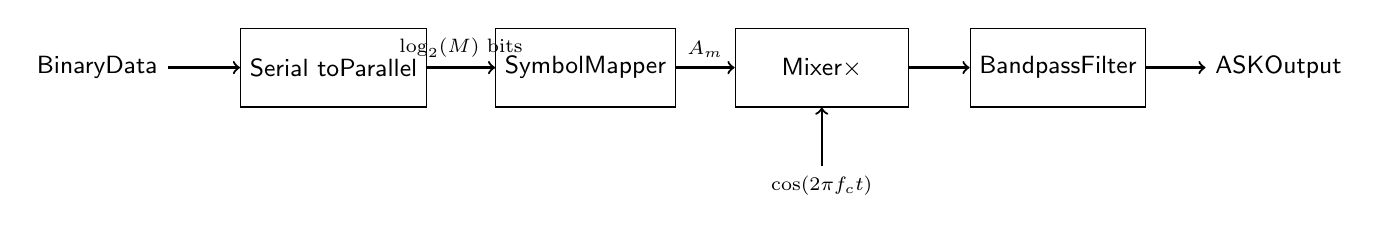
\begin{tikzpicture}[
  block/.style={rectangle, draw, minimum width=2.2cm, minimum height=1cm, font=\sffamily\small},
  node distance=2.2cm,
  font=\small
]
\node (input) {\sffamily Binary\\Data};
\node[block, right of=input, node distance=3cm] (s2p) {Serial to\\Parallel};
\node[block, right of=s2p, node distance=3.2cm] (map) {Symbol\\Mapper};
\node[block, right of=map, node distance=3cm] (mult) {Mixer\\$\times$};
\node[block, right of=mult, node distance=3cm] (filter) {Bandpass\\Filter};
\node[right of=filter, node distance=2.8cm] (output) {\sffamily ASK\\Output};

\node[below of=mult, node distance=1.5cm, font=\scriptsize] (carrier) {$\cos(2\pi f_c t)$};

\draw[->,thick] (input) -- (s2p);
\draw[->,thick] (s2p) -- node[above,font=\scriptsize] {$\log_2(M)$ bits} (map);
\draw[->,thick] (map) -- node[above,font=\scriptsize] {$A_m$} (mult);
\draw[->,thick] (carrier) -- (mult);
\draw[->,thick] (mult) -- (filter);
\draw[->,thick] (filter) -- (output);
\end{tikzpicture}
\end{center}

\textbf{Modulation process:}
\begin{enumerate}
\item \textbf{Serial-to-parallel conversion:} Group incoming bits into symbols of $\log_2(M)$ bits each
\item \textbf{Symbol mapping:} Map bit pattern to amplitude level $A_m$
\item \textbf{Multiply by carrier:} $s(t) = A_m \cos(2\pi f_c t)$
\item \textbf{Pulse shaping:} Apply bandpass filter to:
  \begin{itemize}
  \item Limit occupied bandwidth
  \item Reduce intersymbol interference (ISI)
  \item Meet spectral mask requirements
  \end{itemize}
\end{enumerate}

\subsection{Receiver (Coherent Detector)}

Coherent detection requires a phase-synchronized local oscillator:

\begin{center}
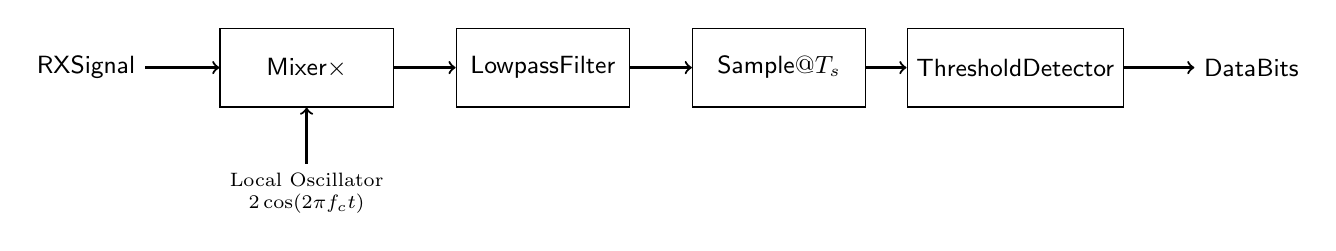
\begin{tikzpicture}[
  block/.style={rectangle, draw, minimum width=2.2cm, minimum height=1cm, font=\sffamily\small},
  node distance=2.2cm,
  font=\small
]
\node (input) {\sffamily RX\\Signal};
\node[block, right of=input, node distance=2.8cm] (mult) {Mixer\\$\times$};
\node[block, right of=mult, node distance=3cm] (lpf) {Lowpass\\Filter};
\node[block, right of=lpf, node distance=3cm] (sample) {Sample\\$@T_s$};
\node[block, right of=sample, node distance=3cm] (thresh) {Threshold\\Detector};
\node[right of=thresh, node distance=3cm] (output) {\sffamily Data\\Bits};

\node[below of=mult, node distance=1.6cm, font=\scriptsize, align=center] (lo) {Local Oscillator\\$2\cos(2\pi f_c t)$};

\draw[->,thick] (input) -- (mult);
\draw[->,thick] (lo) -- (mult);
\draw[->,thick] (mult) -- (lpf);
\draw[->,thick] (lpf) -- (sample);
\draw[->,thick] (sample) -- (thresh);
\draw[->,thick] (thresh) -- (output);
\end{tikzpicture}
\end{center}

\textbf{Detection process:}
\begin{enumerate}
\item \textbf{Multiply by local carrier:}
\begin{equation}
r(t) = A_m \cos(2\pi f_c t) \cdot 2\cos(2\pi f_c t) = A_m[1 + \cos(4\pi f_c t)]
\end{equation}

\item \textbf{Lowpass filter} removes $2f_c$ component:
\begin{equation}
y(t) = A_m + n(t)
\end{equation}
where $n(t)$ is additive white Gaussian noise (AWGN)

\item \textbf{Sample at symbol rate} $T_s$: obtain $y_k = A_m + n_k$

\item \textbf{Threshold detection:} Compare $y_k$ to $(M-1)$ decision thresholds
\begin{equation}
\text{Threshold}_k = \frac{A_k + A_{k+1}}{2}, \quad k = 0, 1, \ldots, M-2
\end{equation}
\end{enumerate}

For 4-ASK, thresholds are placed at $A/2$, $3A/2$, and $5A/2$.

\subsection{Non-Coherent Detection (Envelope Detector)}

For binary ASK (OOK), a simpler non-coherent receiver can be used:

\begin{center}
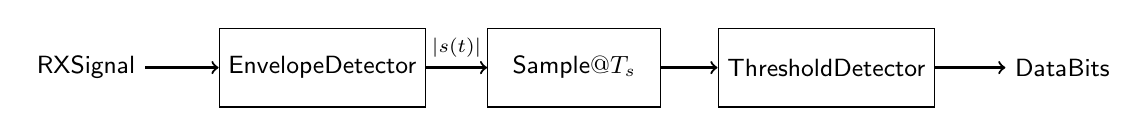
\begin{tikzpicture}[
  block/.style={rectangle, draw, minimum width=2.2cm, minimum height=1cm, font=\sffamily\small},
  node distance=2.2cm,
  font=\small
]
\node (input) {\sffamily RX\\Signal};
\node[block, right of=input, node distance=3cm] (env) {Envelope\\Detector};
\node[block, right of=env, node distance=3.2cm] (sample) {Sample\\$@T_s$};
\node[block, right of=sample, node distance=3.2cm] (thresh) {Threshold\\Detector};
\node[right of=thresh, node distance=3cm] (output) {\sffamily Data\\Bits};

\draw[->,thick] (input) -- (env);
\draw[->,thick] (env) -- node[above,font=\scriptsize] {$|s(t)|$} (sample);
\draw[->,thick] (sample) -- (thresh);
\draw[->,thick] (thresh) -- (output);
\end{tikzpicture}
\end{center}

\textbf{Envelope detector:} Rectifier followed by lowpass filter to extract signal magnitude $|s(t)|$

\textbf{Advantages:}
\begin{itemize}
\item[\checkmark] Simple circuit (no carrier recovery needed)
\item[\checkmark] Low complexity, low cost
\item[\checkmark] Suitable for RFID and IR remote applications
\end{itemize}

\textbf{Disadvantages:}
\begin{itemize}
\item[\texttimes] Approximately 3~dB worse performance than coherent detection
\item[\texttimes] Only practical for binary ASK (OOK)
\item[\texttimes] More sensitive to noise
\end{itemize}

\section{Carrier Recovery}

Coherent ASK detection requires the receiver to generate a local oscillator that is frequency and phase synchronized with the transmitter carrier.

\subsection{Carrier Recovery Techniques}

\subsubsection{1. Pilot Tone}
\begin{itemize}
\item[\checkmark] Simple implementation
\item[\checkmark] Accurate phase reference
\item[\texttimes] Wastes power (typically 10--20\% of total)
\item[\texttimes] Reduces data throughput
\end{itemize}

\subsubsection{2. Costas Loop}
PLL-based carrier recovery using I/Q demodulation:
\begin{itemize}
\item[\checkmark] No pilot tone required
\item[\checkmark] Works for amplitude modulation with modifications
\item[\texttimes] Complex analog circuitry
\item[\texttimes] Acquisition time required
\end{itemize}

\subsubsection{3. Squaring Loop}
Exploits the periodicity of the modulated signal:
\begin{itemize}
\item[\checkmark] Removes data modulation
\item[\checkmark] Robust in low SNR
\item[\texttimes] Phase ambiguity issues
\item[\texttimes] Requires post-processing
\end{itemize}

\subsection{Non-Coherent Alternative}

For binary ASK (OOK), non-coherent envelope detection avoids carrier recovery complexity at the cost of approximately 3~dB performance penalty. This trade-off makes envelope detection attractive for simple, low-cost applications like RFID tags and IR remotes.

\section{Signal Space Representation}

ASK signals form a one-dimensional constellation on the real axis:
\begin{equation}
s_m(t) = A_m \phi(t)
\end{equation}
where $\phi(t) = \sqrt{\frac{2}{T_s}} \cos(2\pi f_c t)$ is the orthonormal basis function.

\subsection{Energy Calculations}

\textbf{Energy per symbol:}
\begin{equation}
E_m = \int_0^{T_s} s_m^2(t) \, dt = \frac{A_m^2 T_s}{2}
\end{equation}

\textbf{Average symbol energy} (assuming equiprobable symbols):
\begin{equation}
\bar{E}_s = \frac{1}{M} \sum_{m=0}^{M-1} E_m = \frac{T_s}{2M} \sum_{m=0}^{M-1} A_m^2
\end{equation}

\textbf{Energy per bit:}
\begin{equation}
E_b = \frac{\bar{E}_s}{\log_2(M)}
\end{equation}

\section{Bit Error Rate (BER) Performance}

\subsection{Coherent Detection in AWGN Channel}

For M-ary ASK with coherent detection, the symbol error rate is:
\begin{equation}
P_s \approx 2\left(1 - \frac{1}{M}\right) Q\left(\sqrt{\frac{6\log_2(M)}{M^2 - 1} \cdot \frac{E_b}{N_0}}\right)
\end{equation}
where:
\begin{itemize}
\item $E_b$ = energy per bit (joules)
\item $N_0$ = noise power spectral density (W/Hz)
\item $Q(x) = \frac{1}{\sqrt{2\pi}}\int_x^\infty e^{-t^2/2}\,dt$ (Gaussian Q-function)
\end{itemize}

Assuming Gray coding, the bit error rate is approximately:
\begin{equation}
\mathrm{BER} \approx \frac{P_s}{\log_2(M)} = \frac{2}{M\log_2(M)}\left(1 - \frac{1}{M}\right) Q\left(\sqrt{\frac{6\log_2(M)}{M^2 - 1} \cdot \frac{E_b}{N_0}}\right)
\end{equation}

\subsection{Performance Benchmarks}

At $E_b/N_0 = 10$~dB:

\begin{center}
\begin{tabular}{@{}lrl@{}}
\toprule
Modulation & \multicolumn{1}{c}{BER} & Observation \\
\midrule
2-ASK (OOK) & $3.9 \times 10^{-6}$ & 1 error in 250,000 bits \\
4-ASK & $1.8 \times 10^{-3}$ & 1 error in 556 bits \\
8-ASK & $\sim 10^{-2}$ & 1 error in 100 bits \\
\bottomrule
\end{tabular}
\end{center}

\begin{keyconcept}
\textbf{Why does BER degrade with higher M?}

As $M$ increases, amplitude levels become closer together ($\Delta A$ decreases for fixed power). This makes the constellation more sensitive to noise. Each doubling of $M$ requires approximately 3--4~dB more $E_b/N_0$ to maintain the same BER.
\end{keyconcept}

\subsection{Required $E_b/N_0$ for Target BER}

For BER $= 10^{-6}$:

\begin{center}
\begin{tabular}{@{}lll@{}}
\toprule
Modulation & Required $E_b/N_0$ (dB) & Penalty vs 2-ASK \\
\midrule
2-ASK (OOK) & 10.5 & Baseline \\
4-ASK & 14.0 & +3.5~dB \\
8-ASK & 18.0 & +7.5~dB \\
16-ASK & 22.0 & +11.5~dB \\
\bottomrule
\end{tabular}
\end{center}

\textbf{Pattern:} Each doubling of $M$ adds approximately 3.5--4~dB penalty.

\section{Bandwidth Efficiency}

The occupied bandwidth with raised-cosine pulse shaping is:
\begin{equation}
B = (1 + \alpha) R_s
\end{equation}
where:
\begin{itemize}
\item $R_s$ = symbol rate (symbols/sec)
\item $\alpha$ = roll-off factor (typically 0.35)
\end{itemize}

Since the bit rate is:
\begin{equation}
R_b = R_s \log_2(M)
\end{equation}

The spectral efficiency becomes:
\begin{equation}
\eta = \frac{R_b}{B} = \frac{\log_2(M)}{1 + \alpha} \quad \text{(bits/sec/Hz)}
\end{equation}

\subsection{Spectral Efficiency Comparison}

For $\alpha = 0.35$:

\begin{center}
\begin{tabular}{@{}llll@{}}
\toprule
Modulation & Bits/symbol & $\eta$ (bps/Hz) & Bandwidth Efficiency \\
\midrule
2-ASK & 1 & 0.74 & Baseline \\
4-ASK & 2 & 1.48 & $2\times$ better \\
8-ASK & 3 & 2.22 & $3\times$ better \\
16-ASK & 4 & 2.96 & $4\times$ better \\
\bottomrule
\end{tabular}
\end{center}

\textbf{Trade-off:} Higher spectral efficiency requires higher SNR to maintain acceptable BER.

\section{Power Efficiency}

\textbf{Average power:}
\begin{equation}
\bar{P} = \frac{1}{M} \sum_{m=0}^{M-1} \frac{A_m^2}{2}
\end{equation}

\textbf{Peak-to-average power ratio (PAPR):}
\begin{equation}
\mathrm{PAPR} = \frac{A_{\max}^2}{\bar{P}}
\end{equation}

For M-ASK with equally-spaced amplitudes $\{0, A, 2A, \ldots, (M-1)A\}$:
\begin{equation}
\mathrm{PAPR} = \frac{3(M-1)}{2M-1}
\end{equation}

\begin{warningbox}
High PAPR stresses power amplifiers, requiring significant backoff to avoid nonlinear distortion. This reduces overall transmitter efficiency.
\end{warningbox}

\section{Comparison with Other Modulation Schemes}

At the same bit rate and $E_b/N_0 = 10$~dB:

\begin{center}
\begin{tabular}{@{}lllll@{}}
\toprule
Modulation & Bits/symbol & Constellation & BER & Notes \\
\midrule
BPSK & 1 & 2 points (1D) & $3.9 \times 10^{-6}$ & Optimal for $M=2$ \\
2-ASK (OOK) & 1 & 2 points (1D) & $3.9 \times 10^{-6}$ & Same as BPSK \\
QPSK & 2 & 4 points (2D) & $3.9 \times 10^{-6}$ & $2\times$ efficiency \\
4-ASK & 2 & 4 points (1D) & $1.8 \times 10^{-3}$ & Much worse BER \\
16-QAM & 4 & 16 points (2D) & $\sim 10^{-4}$ & Better than 16-ASK \\
16-ASK & 4 & 16 points (1D) & $\sim 10^{-2}$ & Worst BER \\
\bottomrule
\end{tabular}
\end{center}

\begin{keyconcept}
\textbf{Why does QAM outperform ASK for $M > 2$?}

QAM uses a 2D constellation (both I and Q axes), allowing greater separation between constellation points for the same average power. ASK uses only 1D (I-axis only), resulting in tighter symbol spacing and worse noise immunity. This fundamental geometric advantage makes QAM the preferred choice for RF communications when $M > 2$.
\end{keyconcept}

\section{Practical Implementations}

\subsection{Fiber Optic Communications}

Binary ASK (On-Off Keying) dominates short-reach optical links:

\begin{itemize}
\item \textbf{10 Gigabit Ethernet (10GBASE-SR/LR):} OOK with direct detection
\item \textbf{Passive Optical Networks (PON):} OOK for upstream transmission
\item \textbf{Implementation:} Laser ON/OFF modulation, photodiode detection
\item \textbf{Data rate:} 1--100~Gbps depending on generation
\end{itemize}

\textbf{Higher-order ASK:} PAM-4 (4-ASK) is emerging for 100G+ applications:
\begin{itemize}
\item 50~Gbaud PAM-4 = 100~Gbps (2 bits/symbol)
\item Used in 400G Ethernet (4$\times$100G lanes)
\item Trade-off: Higher spectral efficiency vs increased SNR requirement
\end{itemize}

\subsection{RFID Systems}

Passive RFID tags use backscatter modulation with OOK:

\begin{itemize}
\item \textbf{Reader$\rightarrow$Tag:} Continuous carrier provides power
\item \textbf{Tag$\rightarrow$Reader:} Load modulation (reflection vs absorption)
\item \textbf{Frequencies:} 125~kHz (LF), 13.56~MHz (HF), 900~MHz (UHF)
\item \textbf{Data rate:} 40--640~kbps (EPC Gen2 standard)
\item \textbf{Range:} 10~cm (HF) to 10~m (UHF)
\end{itemize}

\textbf{Advantage:} Non-coherent detection enables extremely simple tag circuitry with minimal power consumption.

\subsection{Infrared Remote Controls}

Consumer electronics use OOK at 38~kHz carrier frequency:

\begin{itemize}
\item \textbf{Protocol:} Manchester-encoded OOK
\item \textbf{Range:} 5--10 meters (line-of-sight)
\item \textbf{Power:} $<$10~mW (eye safety)
\item \textbf{Receiver:} Simple envelope detector with bandpass filter
\end{itemize}

\subsection{Visible Light Communication (VLC)}

LED-based VLC systems use intensity modulation (OOK or M-ASK):

\begin{itemize}
\item \textbf{Data rate:} 100+~Mbps with OOK
\item \textbf{Dimming support:} Adjust average amplitude (DC bias)
\item \textbf{Applications:} Indoor positioning, Li-Fi broadband
\item \textbf{Advantage:} Simultaneous illumination and data transmission
\end{itemize}



\section{Implementation Challenges}

\subsection{Automatic Gain Control (AGC)}

\begin{warningbox}
Received signal amplitude varies due to path loss, fading, and shadowing. For M-ASK with $M > 2$, \textbf{precise AGC is critical} to maintain threshold accuracy. AGC errors directly translate to increased BER.
\end{warningbox}

The AGC adjusts receiver gain to maintain constant signal level:
\begin{equation}
\text{Gain}(t) = \frac{A_{\text{target}}}{\hat{A}_{\text{received}}(t)}
\end{equation}

\subsection{Nonlinear Distortion}

Power amplifier nonlinearity compresses high amplitude levels, causing:
\begin{itemize}
\item Unequal spacing between constellation points
\item Increased symbol error rate
\item Spectral regrowth
\end{itemize}

\textbf{Mitigation strategies:}
\begin{itemize}
\item \textbf{Backoff:} Operate PA below saturation (reduces efficiency)
\item \textbf{Predistortion:} Digital or analog linearization techniques
\item \textbf{Alternative:} Use constant-envelope modulation (PSK, FSK)
\end{itemize}

\subsection{Fading Channels}

ASK is particularly vulnerable to fading because amplitude directly carries information:
\begin{equation}
r(t) = h(t) \cdot s(t) + n(t)
\end{equation}

where fading coefficient $|h(t)|$ multiplies the signal amplitude, potentially causing severe performance degradation.

\textbf{Mitigation:}
\begin{itemize}
\item Channel equalization to compensate for fading
\item OFDM to convert frequency-selective fading to flat fading per subcarrier
\item Consider phase-based modulation (PSK) for fading channels
\end{itemize}

\section{Worked Example: Fiber Optic Link}

\textbf{Scenario:} 10~Gbps OOK fiber optic link with direct detection

\subsection*{Given Parameters}

\begin{tabular}{@{}ll@{}}
Data rate & $R_b = 10$~Gbps \\
Laser power & $P_t = 0$~dBm = 1~mW \\
Fiber loss & 0.2~dB/km \\
Link distance & $L = 10$~km \\
Receiver sensitivity & $-28$~dBm (for BER $= 10^{-12}$) \\
Connector losses & 1~dB (2 connectors $\times$ 0.5~dB) \\
\end{tabular}

\subsection*{Step 1: Total Link Loss}

\begin{equation}
L_{\text{total}} = L_{\text{fiber}} + L_{\text{connectors}} = (0.2 \times 10) + 1 = 3~\text{dB}
\end{equation}

\subsection*{Step 2: Received Power}

\begin{equation}
P_r = P_t - L_{\text{total}} = 0 - 3 = -3~\text{dBm}
\end{equation}

\subsection*{Step 3: Link Margin}

\begin{equation}
\text{Margin} = P_r - P_{\text{sensitivity}} = -3 - (-28) = 25~\text{dB}
\end{equation}

\begin{calloutbox}[colback=black!8!white,colframe=black]{Link Budget Summary}
\textbf{Result: Link closes with 25~dB margin}

This comfortable margin accommodates:
\begin{itemize}
\item Fiber aging and macrobending losses ($\sim$5~dB)
\item Temperature variations ($\sim$2--3~dB)
\item Component degradation over lifetime
\item Safety factor for repairs/splices
\end{itemize}

\textbf{Conclusion:} Link is highly viable for 10~Gbps OOK transmission over 10~km with excellent reliability margin.
\end{calloutbox}

\section{Advantages and Disadvantages}

\subsection*{Advantages}

\begin{enumerate}
\item \textbf{Simple implementation:} Single mixer, no quadrature components
\item \textbf{Non-coherent detection possible:} Envelope detector for OOK (no carrier recovery)
\item \textbf{Low cost:} Minimal hardware complexity suitable for RFID and IR remotes
\item \textbf{Ideal for optical systems:} Directly compatible with intensity modulation (lasers/LEDs)
\end{enumerate}

\subsection*{Disadvantages}

\begin{enumerate}
\item \textbf{Poor power efficiency:} 1D constellation gives worse BER than 2D schemes (QAM, PSK)
\item \textbf{Highly susceptible to fading:} Amplitude fluctuations directly corrupt information
\item \textbf{Nonlinear amplifier sensitivity:} High PAPR causes distortion in power amplifiers
\item \textbf{Requires accurate AGC:} Critical for $M > 2$ to maintain threshold accuracy
\item \textbf{Inferior to alternatives:} For $M > 2$ in RF, QAM/PSK strongly preferred
\end{enumerate}

\section{Summary}

\begin{center}
\begin{tabular}{@{}ll@{}}
\toprule
\textbf{Parameter} & \textbf{Value} \\
\midrule
Bits per symbol & $\log_2(M)$ \\
Constellation dimensionality & 1D (I-axis only) \\
Spectral efficiency (2-ASK) & $\sim$0.7--1.0~bps/Hz \\
Spectral efficiency (M-ASK) & $\sim\log_2(M)/(1+\alpha)$~bps/Hz \\
BER @ 10~dB $E_b/N_0$ (2-ASK) & $3.9 \times 10^{-6}$ \\
BER @ 10~dB $E_b/N_0$ (4-ASK) & $1.8 \times 10^{-3}$ \\
Carrier recovery & Required for coherent (not for OOK envelope) \\
Implementation complexity & Low (simple) \\
Best application & Optical communications, RFID \\
Typical uses & Fiber optics, RFID, IR remotes, VLC \\
\bottomrule
\end{tabular}
\end{center}

\section{Further Reading}

\begin{itemize}
\item \textbf{Chapter 5:} On-Off Keying (OOK)---binary ASK implementation details
\item \textbf{Chapter 6:} Frequency-Shift Keying (FSK)---alternative binary modulation
\item \textbf{Chapter 7:} Binary Phase-Shift Keying (BPSK)---phase-based alternative
\item \textbf{Chapter 8:} Quadrature Phase-Shift Keying (QPSK)---2D phase modulation
\item \textbf{Chapter 9:} Quadrature Amplitude Modulation (QAM)---superior 2D scheme
\item \textbf{Chapter 12:} Constellation Diagrams---signal space visualization
\item \textbf{Chapter 13:} IQ Representation---complex baseband analysis
\item \textbf{Chapter 18:} Bit Error Rate Analysis---performance metrics and theory
\item \textbf{Chapter 25:} Carrier Recovery Techniques---synchronization methods
\end{itemize}
